\documentclass[a4paper,11pt,german,notitlepage]{report}
\usepackage{xcolor}
\usepackage{tabularx}
\usepackage{dclecture}
\usepackage{qrcode}
\usepackage{awesomebox}
\usepackage{circuitikz}
\usepackage[style=german, german=swiss]{csquotes}
\def\farbe{darkgray} %Hier Farbe definieren
\addbibresource{refs.bib}

\ctikzset{
    logic ports=ieee,
    logic ports/scale=0.8,
    logic ports/fill=lightgray
}

\usetikzlibrary{arrows,shapes.gates.logic.US,shapes.gates.logic.IEC,calc,positioning}

\graphicspath{{img/}}

% Extract Exercises

%\usepackage[active, generate=trigonometry_exercises, extract-env={ex}]{extract}
%\begin{extract}
%\usepackage{xcolor}
%\def\farbe{teal}
%\usepackage{dcexercisesnogrid}
%\exercisetrue
%\end{extract}


%%% Fancy Header and Footer
\renewcommand{\headrule}{\vbox to 0pt{\hbox to\headwidth{\color{\farbe}\rule{\headwidth}{1pt}}\vss}}
\pagestyle{fancy} %eigener Seitenstil
\fancyhf{} %alle Kopf- und Fu§zeilenfelder bereinigen
\fancyhead[C]{Informatik - Gymnasium 1. Klasse - Algorithmen Projekt - Mini Solitaire} %Kopfzeile mitte
%\fancyhead[R]{\includegraphics[width=0.2cm]{x.png}}

\fancyfoot[C]{\thepage}

%\rfoot{\setlength{\unitlength}{1mm}
%\begin{picture}(0,0)
%\put(5,0){\includegraphics{pic\thepage.ps}}
%\end{picture}}


\parskip=.1cm
\parindent=0cm
\linespread{1.5}

\begin{document}

\section*{Beschreibung}
Mini Solitaire ist eine vereinfachte Variante des bekannten Kartenspiels Solitaire bei dem es darum geht, gemischte Karten Stück für Stück nach Farben und Kartenwerten zu sortieren.
Ihr Ziel in diesem Projekt ist es, einen Algorithmus zu entwickeln, welcher Mini Solitaire effizient und optimal lösen kann.
\section*{Regeln}
Das Spiel beginnt mit gemischten Karten, welche zufällig auf den ersten zwei Ablageplätzen aufgestapelt sind.
Es gibt Karten zweier Farben: schwarz und rot (später können noch neue Farben hinzukommen).

\begin{description}
    \item[Ziel:] Auf allen Ablageplätzen sollen jeweils alle Karten einer Farbe in absteigender Reihenfolge von oben nach unten aufgestapelt sein.
    \item[Züge:] Sie können jeweils die oberste Karte von einem Stapel wegnehmen. Auf dem Ziel-Ablagestapel muss eine Karte gleicher Farbe und höherem Wert liegen, damit Sie die Karte ablegen dürfen (Bsp.: rote 1 geht auf rote 2, aber nicht auf rote 0). Auf leeren Ablageplätzen dürfen beliebige Karten gespielt werden.
\end{description}
\begin{figure}[h!]
    \centering
    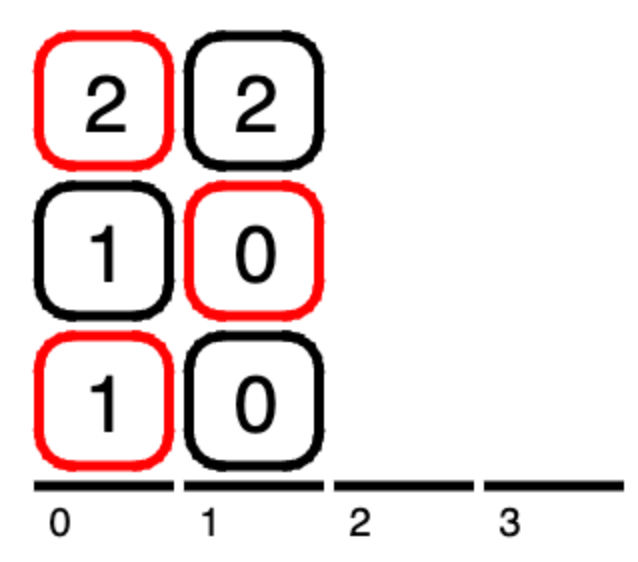
\includegraphics[width=5cm]{mini_solitaire.png}
    \caption{Screenshot von WebTigerJython. Eine mögliche Startsituation im Mini Solitaire. Was wäre hier wohl der schnellste Weg zum Ziel?}
\end{figure}
Als Notation von Zügen für dieses Problem verwenden wir die Position der Ablageplätze.
In der Vorlage haben Sie vier Ablageplätze.
Wir teilen jedem Ablageplatz von links aus eine Zahl beginnend bei $0$ zu.
Die Ablageplätze sind also $0,1,2,3$.\\
Wenn Sie eine Karte von Ablageplatz $1$ zu Ablageplatz $0$ bewegen, wäre die Notation dazu $(1,0)$ (von Platz 1 zu Platz 0).
Eine Karte kann nicht von einem Ablageplatz zum gleichen Ablageplatz gelegt werden, da dann ja der gleiche Zustand erreicht würde.
Das bedeutet, das Beispielsweise der Zug $(0,0)$ nicht relevant ist.
Im oben gezeigten Beispiel gäbe es vier legale Züge: $(0,2),(0,3),(1,2),(1,3)$. Die Züge $(1,0)$ und $(0,1)$ wären nicht legal, da die Farben und Werte nicht aufeinander passen.

Sie beginnen bereits mit einer implementierten Suche in der Codevorlage.
Diese Suche ist jedoch extrem ineffizient.
Nach 4000 durchsuchten Zuständen bricht das Program ab, um Ihren Computer zu schonen.
Es kann also sein, dass die Suche keine Lösung findet.

\section*{Aufgabe}
Hier werden zusätzliche Aufgaben beschrieben, welche spezifisch für Ihr Projekt sind.
Die Aufgaben sind in zwei Gruppen unterzeilt: Pflichtaufgaben und optionale Aufgaben.
Die Pflichtaufgaben sollen am Ende des Projektes beantwortet sein.
Die optionalen Aufgaben dienen dazu, sich weiter im Thema zu vertiefen.
Diese Aufgaben sind Vorschläge. Sie dürfen auch eigene Fragestellungen vertiefen.
Deklarieren Sie Ihre Fragestellungen klar im Projektbericht.
Für alle Projekt gilt natürlich, dass Sie zuerst die allgemeine Aufgabenstellung und den Code (falls vorhanden) verstehen sollten, bevor Sie die untenstehen Aufgaben bearbeiten.
\subsection*{Pflichtaufgaben}
\begin{itemize}
    \item In der Vorlage ist bereits eine Suche Implementiert. Vergleichen Sie diese Suche mit dem manuellen Eingeben einer Lösung. Was fällt auf? Um was für einen Algorithmus könnte es sich handeln?
    \item Schreiben Sie ein Programm (oder verbessern Sie das existierende), welches jeweils eine optimale Lösung für Ihr Problem findet.
    \item Erweitern Sie das Problem, indem Sie die Konfiguration ändern (\textit{max\_cards} und \textit{slot\_count} auf 4 setzen). Finden Sie mit Ihrem Ansatz noch eine Lösung? Begründen Sie.
\end{itemize}
\subsection*{Optionale Aufgaben}
\begin{itemize}
    \item Implementieren Sie eine Heuristik, welcher jedem Zug angibt, wie gut er ist. Begründen Sie, warum Sie Ihre Heuristik gewählt haben.
    \item Implementieren Sie Ihre Heuristik in einem Suchalgorithmus.
    \item Was passiert mit dem Problem, wenn Sie in der Konfiguration eine weitere Farbe \textit{"blue"} hinzufügen?
    \item (Sehr schwierig!) Implementieren Sie eine Suche, welche das Aufheben mehrerer Container in betracht zieht.
\end{itemize}

\end{document}  
